\documentclass{standalone}
\usepackage{mathpazo}
\usepackage{siunitx}
\usepackage[american voltages, american currents, american inductors]{circuitikz}
\usetikzlibrary{calc}
\newcommand*{\equal}{=}

\begin{document}
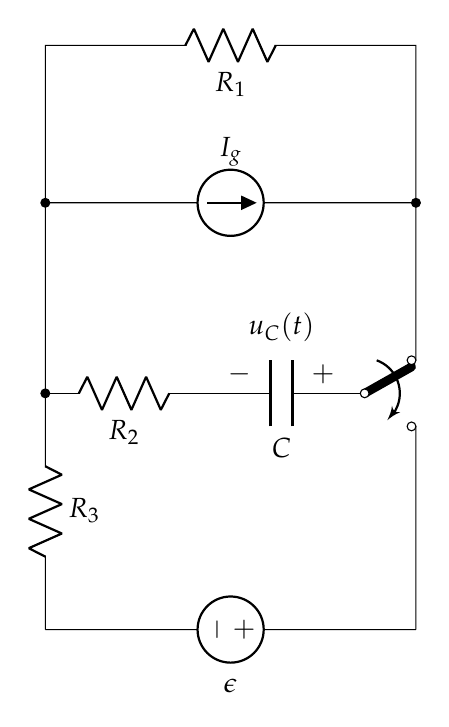
\begin{tikzpicture}
  \draw
  (0,0) node[cute spdt up arrow] (Sw) {};
  \draw
  (Sw.in) to [C, l = $C$, v=$u_C(t)$] ++(-2, 0)
  to [R, l = $R_2$] ++(-2, 0) coordinate (C);
  \draw
  (Sw.out 1) to [short, -*] ++(0, 2) coordinate (F)
  (C|-F) to [isource, l = $I_g$, *-] (F)
  to [short] ++(0, 2) coordinate (E)
  to [R, l = $R_1$] (C|-E)
  to [short, -*] (C)
  to [R, l = $R_3$] ++(0, -3) coordinate (D)
  (Sw.out 2|-D) to [V, v = $\epsilon$] (D)
  (Sw.out 2|-D) to [short] (Sw.out 2);
  \end{tikzpicture}
\end{document}